\documentclass[twocolumn,numberedappendix,trackchanges]{../aastex62}

% these lines seem necessary for pdflatex to get the paper size right
\pdfpagewidth 8.5in
\pdfpageheight 11.0in

% for the red MarginPars
\usepackage{color}

% some extra math symbols
\usepackage{mathtools}

% allows Greek symbols to be bold
\usepackage{bm}

% allows us to force the location of a figure
\usepackage{float}

% allows comment sections
\usepackage{verbatim}

% Override choices in \autoref
\def\sectionautorefname{Section}
\def\subsectionautorefname{Section}
\def\subsubsectionautorefname{Section}

% MarginPars
\setlength{\marginparwidth}{0.75in}
\newcommand{\MarginPar}[1]{\marginpar{\vskip-\baselineskip\raggedright\tiny\sffamily\hrule\smallskip{\color{red}#1}\par\smallskip\hrule}}

\newcommand{\msolar}{\mathrm{M}_\odot}

% Software names
\newcommand{\amrex}{\texttt{AMReX}}
\newcommand{\boxlib}{\texttt{BoxLib}}
\newcommand{\castro}{\texttt{CASTRO}}
\newcommand{\maestro}{\texttt{Maestro}}
\newcommand{\microphysics}{\texttt{Microphysics}}
\newcommand{\wdmerger}{\texttt{wdmerger}}
\newcommand{\python}{\texttt{Python}}
\newcommand{\matplotlib}{\texttt{matplotlib}}
\newcommand{\yt}{\texttt{yt}}
\newcommand{\vode}{\texttt{VODE}}
\newcommand{\isoseven}{\texttt{iso7}}
\newcommand{\aproxthirteen}{\texttt{aprox13}}
\newcommand{\aproxnineteen}{\texttt{aprox19}}
\newcommand{\aproxtwentyone}{\texttt{aprox21}}

\begin{document}

%==========================================================================
% Title
%==========================================================================
\title{Numerical Stability of Detonations in White Dwarf Simulations}

\shorttitle{Numerical Detonations}
\shortauthors{Katz et al. (2018)}

\author{Max P. Katz}
\affiliation
{
  NVIDIA Corporation, 2788 San Tomas Expressway, Santa Clara, CA, 95051, USA
}

\author{Michael Zingale}
\affiliation
{
  Department of Physics and Astronomy, Stony Brook University, Stony Brook, NY, 11794-3800, USA
}



%==========================================================================
% Abstract
%==========================================================================
\begin{abstract}
Some simulations of Type Ia supernovae feature self-consistent thermonuclear
detonations. However, these detonations are not meaningful if the simulations
are not resolved, so it is important to establish an understanding of the
requirements for achieving a numerically converged detonation. In this
study we examine a test detonation problem inspired by collisions of white dwarfs.
This test problem demonstrates that achieving a converged thermonuclear ignition
requires spatial resolution much finer than 1 km in the burning region.
Current computational resource constraints place this stringent resolution
requirement out of reach for multi-dimensional supernova simulations.
Consequently, contemporary simulations that self-consistently demonstrate
detonations are very likely not resolved and should be treated with caution.
\end{abstract}
\keywords{supernovae: general - white dwarfs}

%==========================================================================
% Introduction
%==========================================================================
\section{Introduction}
\label{sec:introduction}

Thermonuclear detonations are common to all current likely models of Type Ia
supernovae (SNe Ia), but how they are actually generated in progenitor systems
is still an open question. Different models predict different locations for
the detonation and different mechanisms for initiating the event. Common to all
of the cases is a severe lack of numerical resolution in the location where the
detonation is expected to occur. The length and time scale at which a detonation
forms is orders of magnitude smaller than the resolution that typical multi-dimensional
hydrodynamic simulations can achieve. The mere presence of a detonation (or lack thereof)
in a simulation is therefore only weak evidence regarding whether a detonation would truly occur.

In this study we examine the challenges associated with simulating thermonuclear detonations.
The inspiration for this work comes from the literature on head-on collisions of WDs,
which can occur, for example, in certain triple star systems \citep{thompson:2011,hamers:2013}.
WD collisions rapidly convert a significant amount of kinetic energy into thermal energy and
thus set up conditions ripe for a thermonuclear detonation. Since they are easy to set up,
they are a useful vehicle for studying the properties of detonations.

Early studies on WD collisions \citep{rosswog:2009,raskin:2010,loren-aguilar:2010,
hawley:2012,garcia-senz:2013} typically had effective spatial resolutions in the
range 100--500 km \added{for the grid codes, and 10--100 km for the SPH codes}, and observed detonations that convert a large amount of
carbon/oxygen material into iron-group elements. These studies varied in methodology
(Lagrangian versus Eulerian evolution, nuclear network used) and did not closely agree
on the final result of the event (see Table 4 of \cite{garcia-senz:2013} for a summary).
\cite{kushnir:2013} argued that many of these simulations featured numerically unstable
evolution, ultimately caused by the zone size being significantly larger than the length
scale over which detonations form. The detonation length scale can vary widely based
on physical conditions \citep{seitenzahl:2009,garg:2017} but is generally \replaced{much
smaller than 100 km}{not larger than 10 km}.

In this paper, we attempt to find what simulation length scale is required to achieve
converged thermonuclear ignitions. \added{In our two-dimensional axisymmetric simulations
of WD collisions, using the Eulerian reactive hydrodynamics code \castro\ \citep{castro, astronum:2017},
the simulations are unresolved at the highest resolution we could afford to run (0.25 km).
So, in this paper we turn to a 1D test, which allows us to test at much higher resolution.}



%==========================================================================
% 1D collision test problem
%==========================================================================
\section{Test Problem}
\label{sec:collisions}

Our test problem is inspired by \cite{kushnir:2013}, and very loosely approximates the
conditions of two $0.64\ \msolar$ WDs colliding head-on. The simulation domain is 1D with a
reflecting boundary at $x = 0$. For $x > 0$ there is a uniform fluid composed (by mass)
of $50\%\, ^{12}$C, $45\%\, ^{16}$O, and $5\%\, ^{4}$He. The fluid is relatively cold,
$T = 10^7$ K, has density $\rho = 5 \times 10^6$ g/cm$^3$, and is traveling toward the
origin with velocity $-2 \times 10^8$ m/s. A uniform constant gravitational acceleration
is applied, $g = -1.1 \times 10^8$ m/s$^{2}$. This setup causes a sharp initial release
of energy at $x = 0$, and the primary question is whether a detonation occurs promptly
near this contact point, or occurs later (possibly at a distance from the contact point).
The simulated domain has width $1.6384 \times 10^9$ cm, and we apply inflow boundary conditions
that keep feeding the domain with material that has the same conditions as the initial fluid.
Simulations are performed with the adaptive mesh refinement (AMR) code \castro.
For the burning we use the alpha-chain nuclear network
\texttt{aprox13}. \deleted{The results we describe below do not strongly depend on the network.}
Release 18.12 of the \castro\ code was used. The \amrex\ and \microphysics\ repositories
that \castro\ depends on were also on release 18.12. The problem is located in the
\texttt{Exec/science/Detonation} directory, and we used the \texttt{inputs-collision} setup.

The simulation is terminated when the peak temperature on the domain first reaches
$4 \times 10^9$ K, which we call a thermonuclear ignition. This stopping criterion is a
proxy for the beginning of a detonation. Reaching this temperature does not guarantee
that a detonation will begin, and in this study we do not directly address the question
of whether a ignition of this kind always leads to a detonation. \added{Nor are we commenting
on the physics of the ignition process itself.} Rather, the main question
we investigate here is whether this ignition is numerically converged, \added{and for this purpose
this arbitrary stopping point is sufficient, since in a converged simulation the stopping point
should be reached at the same time independent of resolution}. A converged ignition
is a prerequisite to having a converged detonation. We measure two diagnostic quantities:
the time since the beginning of the simulation required to reach this ignition criterion,
and the distance from the contact point of the peak temperature.

The only parameter we vary in this study is the spatial resolution used for this problem.
For low resolutions we vary only the base resolution of the grid, up to a resolution of
0.25 km. For resolutions finer than this, we fix the base grid at a resolution of 0.25 km,
and use AMR applied on gradients of the temperature. We tag zones for refinement if the temperature
varies by more than 50\% between two zones. Timesteps are limited only by the hydrodynamic
stability constraint, with CFL number 0.5. Although this leads to Strang splitting error
in the coupling of the burning and hydrodynamics for low resolution, we have verified that
the incorrect results seen at low resolution do not meaningfully depend on the timestep constraint
(both by applying a timestep limiter based on nuclear burning, and by using the spectral deferred
corrections driver in \castro, which directly couples the burning and hydrodynamics). At very high
resolution, the splitting error tends to zero as the CFL criterion decreases the timestep.

\begin{figure}[ht]
  \centering
  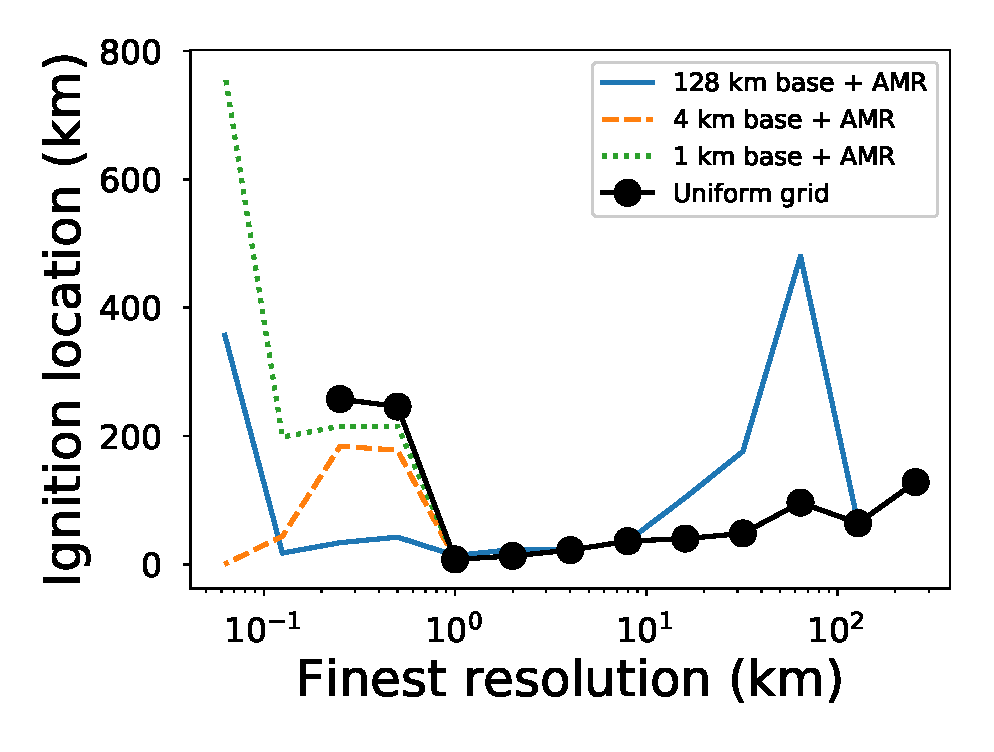
\includegraphics[scale=0.30]{{{plots/amr_ignition_self-heat}}}
  \caption{Distance from the contact point of the ignition (solid blue), and time of the
           ignition (dashed green), as a function of finest spatial resolution.
           \label{fig:self-heat-distance}}
\end{figure}

\autoref{fig:self-heat-distance} shows our main results. The lowest resolution we consider,
256 km, is typical of the early simulations of white dwarf collisions, and demonstrates a
prompt ignition near the contact point. As the (uniform) resolution increases, the ignition
tends to occur earlier and nearer to the contact point. This trend is not physically meaningful:
all simulations with resolution worse than about 1 km represent the same prompt central ignition,
and as the resolution increases, there are grid points physically closer to the center that can ignite.
However, when the resolution is better than 1 km, the situation changes dramatically: the prompt
central ignition does not occur, but rather the ignition is delayed and occurs further from the contact
point. When we have finally \replaced{(perhaps) converged}{reached the point where the curves start to flatten},
the ignition occurs around 900 km from the contact point, about 1 second after contact (contrast to less than
0.05 seconds for the simulation with 1 km resolution). \added{Even at this resolution, it is not clear if
the simulation is converged. We were unable to perform higher resolution simulations to check convergence
due to the length of time that would be required.} This story contains two important lessons. First,
the required resolution for even a qualitatively converged simulation, less than 100 m, is out of reach
of current 3D supernova simulations. Second, the behavior for resolutions worse than 1 km qualitatively
appears to be converged, and one could perhaps be misled into thinking that there was no reason to
try higher resolutions, which is reason for caution in interpreting reacting hydrodynamics simulations.



\section{Numerically Unstable Burning}
\label{sec:unstable_burning}

\citet{kushnir:2013} observe an important possible failure mode
for reacting hydrodynamics simulations. Let us define $\tau_e = e / \dot{e}$
as the nuclear energy injection timescale, and $\tau_s = \Delta x / c_s$
as the sound-crossing time in a zone (where $\Delta x$ is the grid
resolution and $c_s$ is the speed of sound). When the sound-crossing
time is too long, energy is built up in a zone faster than it can be
advected away by pressure waves. \added{This effect generalizes to
Langrangian simulations as well, where $\tau_s$ should be understood
as the timescale for transport of energy to a neighboring fluid element.}
This is of course a problem inherent 
only to numerically discretized systems as the underlying fluid equations
are continuous. This can lead to a numerically seeded detonation
caused by the temperature building up too quickly in the zone; the
detonation may be spurious in this case. If $\tau_s \ll \tau_e$,
we can be confident that a numerically seeded detonation has not
occurred. In practice, we will quantify this requirement as:
\begin{equation}
  \tau_s \leq f_{s}\, \tau_e \label{eq:burning_limiter}
\end{equation}
and require that $f_{s}$ is sufficiently smaller than one.
\citet{kushnir:2013} state that $f_{s} = 0.1$ is a sufficient
criterion for avoiding premature ignitions. \citeauthor{kushnir:2013}
enforced this criterion on their simulations by artificially limiting
the magnitude of the energy release after a burn, and claimed that
this is resulted in more accurate WD collision simulations.

We find that for our test problem (and also the WD collisions we have simulated)
we do observe $\tau_s > \tau_e$; typically the ratio is a factor of 2--5 at
low resolution. This means that an ignition is very likely to occur for numerical
reasons, regardless of whether it would occur for physical reasons. \added{At low
resolution, adding more resolution does not meaningfully improve the ratio of
$\tau_s$ to $\tau_e$ at the point of ignition. The ignition timescale is so short
that virtually all of the energy release occurs in a single timestep even if the
timestep gets shorter due to the CFL limiter. It is only when the resolution gets
sufficiently high that we can simultaneously resolve the energy release over multiple
timesteps and the advection of energy across multiple zones. Even at the highest resolution
we could achieve, about 50 cm, $\tau_s / \tau_e$ was 0.8 at ignition, which is not
sufficiently small to be confident of numerical stability at that resolution.}
We thus investigate whether limiting the energy release of the burn (we will term this
``suppressing'' the burn), as proposed by \citeauthor{kushnir:2013},
is a useful technique for avoiding the prompt detonation. \added{Since the limiter ensures
the inequality in \autoref{eq:burning_limiter} holds by construction, the specific
question to ask is whether the limiter achieves the correct answer and is converged
in cases where the simulation would otherwise be uncorrect or unconverged.}

Before we examine the results, consider a flaw in the application of the limiter:
a physical detonation may \textit{also} occur with the property that, in the detonating
zone, $\tau_s > \tau_e$. For example, consider a region of WD material at uniformly
high temperature, say $5 \times 10^9\ \text{K}$, with an arbitrarily large size,
say a cube with side length 100 km. This region will very likely ignite,
even if it is surrounded by much cooler material. By the time the material on
the edges can advect heat away, the material in the center will have long since
started burning carbon, as the sound crossing time scale is sufficiently large
compared to the energy injection time scale. This is true regardless of whether
the size of this cube corresponds to the spatial resolution in a simulation.
Suppression of the burn in this case is unphysical: if we have a zone matching
these characteristics, the zone should detonate.

When the resolution is low enough, there is a floor on the size of a hotspot,
possibly making such a detonation more likely. This is an unavoidable consequence
of the low resolution; yet, it may be the correct result of the simulation that
was performed. That is, even if large hotspots are unphysical because in reality
the temperature distribution would be smoother, if such a large hotspot \textit{were}
to develop (which is the implicit assumption of a low resolution simulation), then
it would likely detonate. If the results do not match what occurs at higher
resolution, then the simulation is not converged and the results are not reliable.
However, it may also be the case that a higher resolution simulation will yield
similar results, for example because even at the higher resolution, the physical
size of the hotspot stays the same. For this reason, an appeal to the numerical
instability criterion alone is insufficient to understand whether a given ignition
is real.

\begin{figure}[ht]
  \centering
  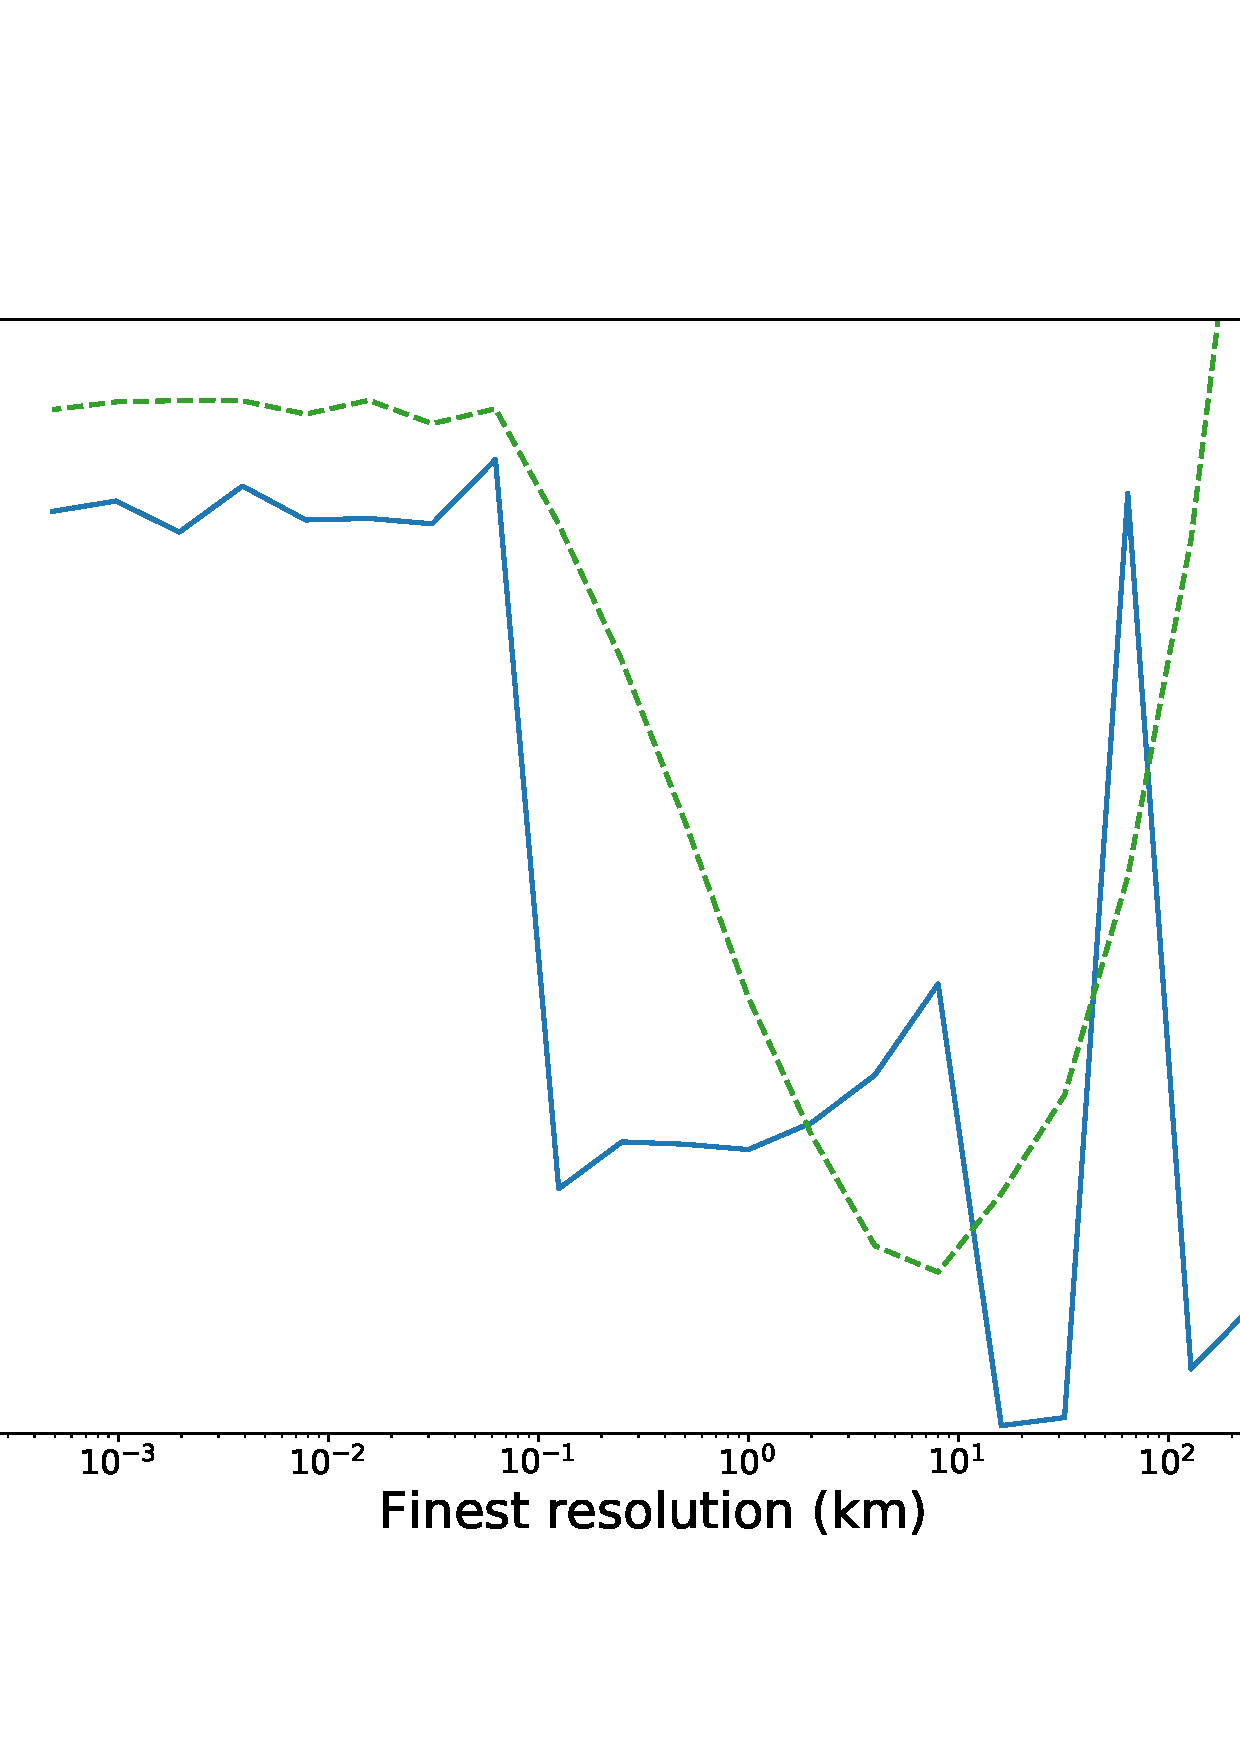
\includegraphics[scale=0.30]{{{plots/amr_ignition_suppressed}}}
  \caption{Similar to \autoref{fig:self-heat-distance}, but for simulations with the
           suppressed burning limiter applied (\autoref{eq:burning_limiter}).
           \label{fig:suppressed-distance}}
\end{figure}

\autoref{fig:suppressed-distance} shows the results we obtain for our implementation of
a ``suppressed'' burning mode. In a suppressed burn, we limit the changes to the state
so that \autoref{eq:burning_limiter} is always satisfied. This is done by rescaling the
energy release and species changes from a burn by a common factor such that the equality
in \autoref{eq:burning_limiter} is satisfied. (If the inequality is already satisfied,
then the integration vector is not modified.) We find that the suppressed burn
generally does not yield correct results for low resolutions. The 64 km resolution
simulation happens to yield approximately the correct ignition distance, but it does
not occur at the right time, and in any case the incorrectness of the results at neighboring
resolutions suggests that this is not a robust finding. The suppressed burning simulation
reaches qualitative convergence at around the same 100 m resolution as the normal self-heating
burn. Because of both the theoretical reasons discussed above, and this empirical finding that
the burning suppression does not make low resolution simulations any more accurate, we do not
believe that the suppressed burning limiter should be applied in production simulations.

\added{To summarize, then, satisfying the stability criterion is neither necessary nor
sufficient, in general, for numerical convergence. It is not necessary because of the
counter-example provided above of a very large hotspot, and it is not sufficient, as the
empirical example in \autoref{fig:suppressed-distance} demonstrates. Nevertheless,
it is a very useful diagnostic metric for understanding simulations, and it is likely
that in many real cases, violation of the stability criterion is a clear sign of
the simulation being under-resolved.}


%==========================================================================
% Conclusions
%==========================================================================
\section{Conclusions and Discussion}\label{Sec:Conclusions and Discussion}
\label{sec:conclusion}

Our example detonation problem demonstrates, at least for this class of
hydrodynamical burning problem, a grid resolution requirement much more stringent
than 1 km. This does not represent all such \added{1D} burning problems: for example, we
have tested similar setups with only carbon and oxygen for which a resolution
in the tens of kilometers is sufficient. \added{However, this should not be construed
as implying that this convergence requirement does not apply to pure C/O WDs.}
\replaced{However}{First}, the fact that it is even possible for
\replaced{this type of burning}{burning in white dwarf material} to require a
resolution better than 100 m should cast significant uncertainty on the results
of simulations featuring detonations that do not meet this resolution
\added{(regardless of the specific conditions). Or, at least, should suggest
that stronger demonstrations of convergence are required. Second, in our real
multi-dimensional simulations of C/O WD collisions, we see the same effect,
where the simulation is not converged even for resolutions up to 0.25 km. It
simply happens to be the case that for the 1D analogue of this problem using pure
C/O the same effect is not seen, which is not particularly surprising since the 1D
setup and the 2D setup are very different and the former lacks any multidimensional
hydrodynamic effects. So we found a related problem that shows a similar
effect in 1D to test convergence at higher resolutions.}

This study does not directly address the problem of how, in the detailed
microphysical sense, a detonation wave actually begins to propagate, as
we cannot resolve this length scale even in our highest resolution simulations.
Rather, we are making the point that for simulations in which a macroscopic
detonation wave appears self-consistently, this is only a valid numerical result
if the resolution is sufficiently high. This convergence requirement does
not imply that the detonation itself is physically realistic; but, it does
imply that we are not even correctly solving the fluid equations we intend
to solve when the convergence requirement is not met. We believe that our
test case can be useful in the future for testing algorithmic innovations
that hope to improve the realism of burning at low resolutions.



\acknowledgments

This research was supported by NSF award AST-1211563 and DOE/Office of
Nuclear Physics grant DE-FG02-87ER40317 to Stony Brook. An award of
computer time was provided by the Innovative and Novel Computational
Impact on Theory and Experiment (INCITE) program.  This research used
resources of the Oak Ridge Leadership Computing Facility located in
the Oak Ridge National Laboratory, which is supported by the Office of
Science of the Department of Energy under Contract
DE-AC05-00OR22725. Project AST106 supported use of the ORNL/Titan
resource.  This research used resources of the National Energy
Research Scientific Computing Center, which is supported by the Office
of Science of the U.S. Department of Energy under Contract
No. DE-AC02-05CH11231. The authors would like to thank Stony Brook
Research Computing and Cyberinfrastructure, and the Institute for
Advanced Computational Science at Stony Brook University for access
to the high-performance LIred and SeaWulf computing systems, the latter
of which was made possible by a \$1.4M National Science Foundation grant (\#1531492).

The authors thank Chris Malone and Don Willcox for useful discussions
on the nature of explosive burning, and Doron Kushnir for providing
clarification on the nature of the burning limiter used in \cite{kushnir:2013}.

This research has made use of NASA's Astrophysics Data System 
Bibliographic Services.

\facility{OLCF}

\bibliographystyle{../aasjournal}
\bibliography{../refs}

\end{document}
